\section{Beispiele}
Auf Grund seines eher einfachen Entscheidungsbaums ist es nicht sehr aufwendig den Algorithmus in einer entsprechenden Programmiersprache wie C zu implementieren. Eine Schleife mit den richtigen if-else-Abfragen und man hat einen funktionierenden Simplex-Downhill programmiert.\\
Nat"urlich ist der Algorithmus auch in Matlab integriert, man kann ihn mittels der Funktion \textbf{fminsearch} aufrufen. 
Der einfachste Aufruf erfolgt, indem man der Funktion \textbf{fminsearch} die Zielfunktion \textbf{fun} sowie den Startwert \textbf{$x_0$} "ubergibt. Wobei der R"uckgabewert ein neuen x-Wert ist, welcher den Funktionswert $fun(x)$ kleiner werden l"asst. 
\begin{lstlisting}
	x = fminsearch(fun,x0)
\end{lstlisting} 
Will man nun beispielsweise beobachten, wie der Algorithmus das Minima sucht, kann man folgenden Code verwenden: 
\newpage
\begin{lstlisting}[style=Matlab]
%------------------------------------------------------------
%Initialisierung
%------------------------------------------------------------
xBorder = 10; 
teration = 20; 
x = (-xBorder:0.1:xBorder);     %Dimensionen x und y
y = (-xBorder:0.1:xBorder); 

[xx, yy] = meshgrid(x,y);       %meshgrid fuer spaetere Ausgabe
Fun = FUNKTION_SEINER_WAHL(xx,yy); %Berechne Funktionswerte

x_newFun = [4.9,4.9];           %Startwert
z_newFun = 0;                   %Funktionswert
x_Fun = zeros(2,2*teration+1);  %Vektor f"ur x1,x2
z_Fun = zeros(1,2*teration+1);  %Vektor f"ur Funktionswerte
options = struct('MaxIter',3);  %Einstellungen fminsearch
%------------------------------------------------------------
%Berechnung Simplex-Downhill
%------------------------------------------------------------
for i=1:(2*teration+1)
	[x_newFun z_newFun] = fminsearch(@FUNKTION_SEINER_WAHL,x_newFun,options2);
	x_Fun(1,i) = x_newFun(1,1);
	x_Fun(2,i) = x_newFun(1,2); 
	z_Fun(i)   = z_newFun; 
end
%------------------------------------------------------------
%Ausgabe Resultate
%------------------------------------------------------------
%Darstellung mittels H"ohenlinien
figure; 
contour(xx,yy,Fun,50);      %Zahl am Ende gibt an, wieviele 
                            %H"ohenlinien geplottet werden
hold on; 
for i=1:length(x_Fun)       %For-Schleife f"ur Visualisierung
    plot(x_Fun(1,i),x_Fun(2,i),'-*r'); 
    pause(0.5)              %Pause von 0.5 Sekunden
end
hold off; 

%Darstellung in 3D
figure; 
mesh(xx,yy,Fun);
hold on; 
plot3(x_Fun(1,:),x_Fun(2,:),z_Fun(:),'r','linewidth',4); 
hold off; 
grid on; 
\end{lstlisting}
Mittels dem in der Initialisierung definierten Struct kann man der Funktion einige Optionen "ubergeben. 
In diesem Fall wird dem Algorithmus mitgeteilt, wieviele Iterationen er pro Aufruf durchf"uhren soll. 
Wenn man - wie in unserem Fall - die Werte beobachten will, so sollte diese Zahl m"oglichst klein sein, darf jedoch nicht kleiner als 2 sein (warum auch immer).
Im folgenden wurde der Code auf die Himmelblau-Funktion angewendet: 
\begin{equation}
	f_{hb} = (x_1^2 + x_2 -11)^2 + (x_1+x_2^2-7)^2
\end{equation}
Diese Funktion hat 4 globale Minima: 
\begin{subequations}
	\begin{align}
		f(3,2) &= 0 \\
		f(-2.81,3.13) &= 0\\
		f(-3.78,-3.28) &= 0\\
		f(3.58,-1.85) &= 0
	\end{align}
\end{subequations}
Auf die Funktion wurden zwei Simplex los gelassen, je in gegen"uberliegenden Ecken (9,9) und (-9,-9).\\
Man sieht deutlich, dass beide Simplexe das ihnen n"achstgelegene Minima ansteuern. 
\begin{figure}[h]
	\centering
	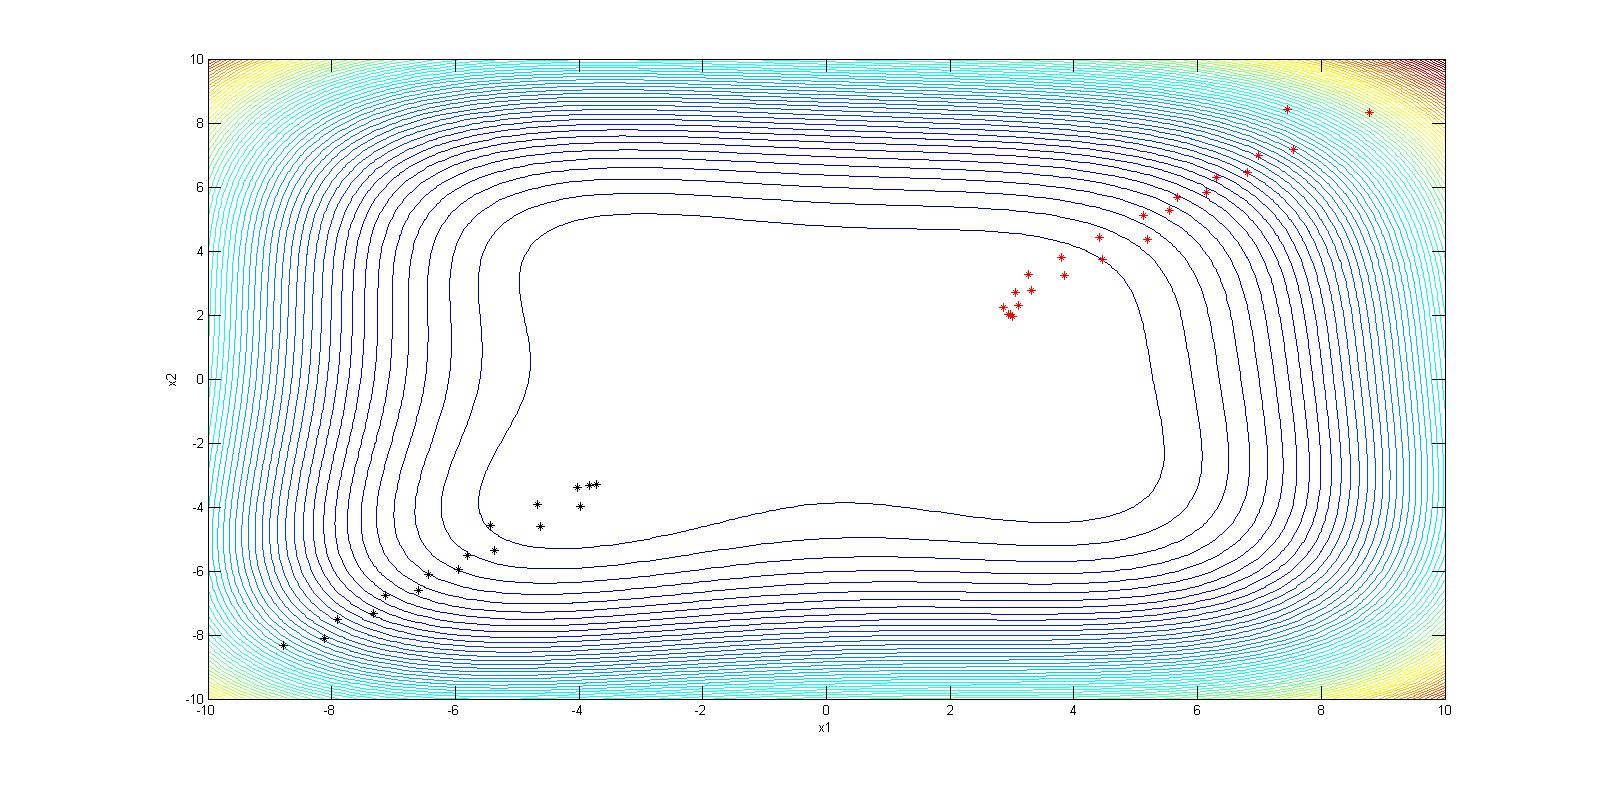
\includegraphics[width=0.8\textwidth]{downhill/HimmelblauHoehen.jpg}%
  	\caption{Simplexe auf Himmelblau-Funktion}%
	\label{fig:HB1}%
\end{figure}


\begin{figure}[htb]
\centering
\begin{subfigure}[b]{0.49\textwidth}
\centering
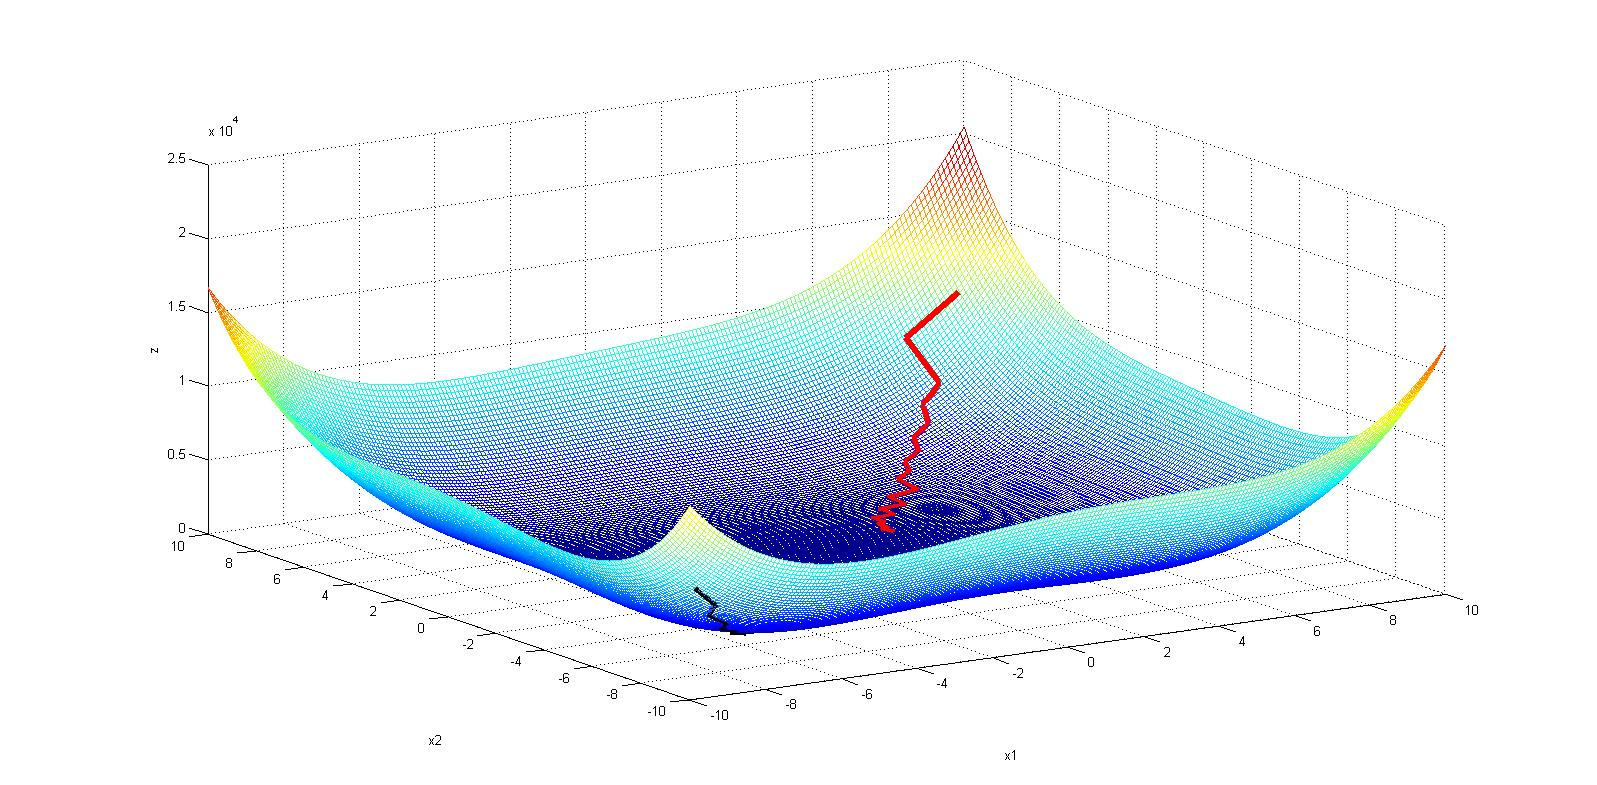
\includegraphics[width=\textwidth]{downhill/Himmelblau3DRot.jpg}
\caption{Rotes Simplex}
\end{subfigure} \begin{subfigure}[b]{0.49\textwidth}
\centering
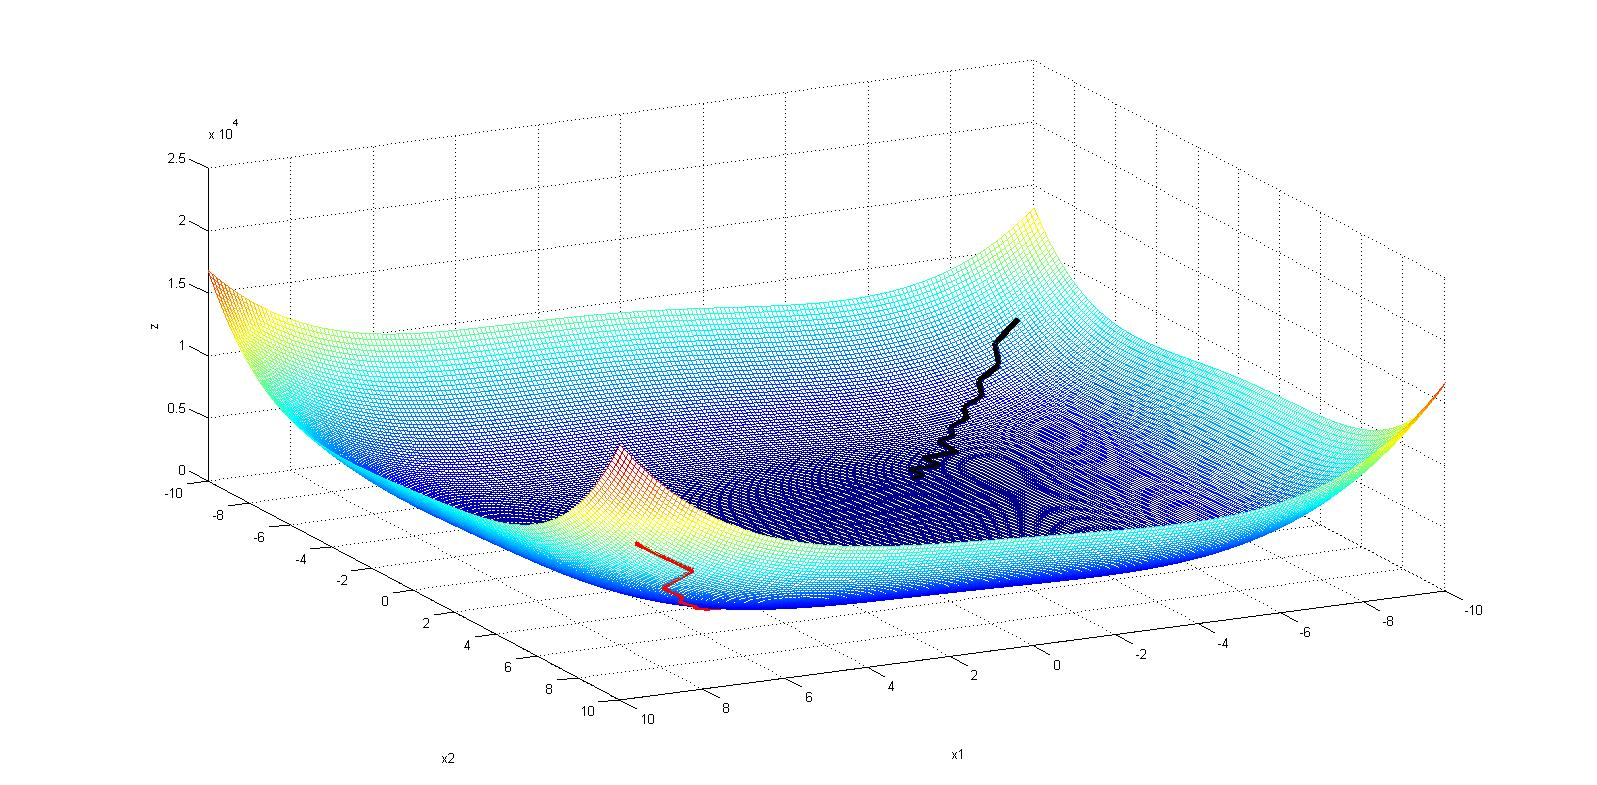
\includegraphics[width=\textwidth]{downhill/Himmelblau3DSchwarz.jpg}
\caption{Schwarzes Simplex}
\end{subfigure}
\caption{Simplex auf Himmelblaufunktion in 3D}
\label{fig:Himmelblau}
\end{figure}



Beim folgenden Bild sieht man, wie der Algorithmus auf die Quadratfunktion angewendet wird, die interne Iterationszahl von \textbf{fminsearch} ist dabei auf 2 gesetzt und der Algorithmus wird 20 mal durchgef"uhrt.

In der Graphik sieht man, dass der Algorithmus eher langsam konvergiert, jedoch von beiden Seiten her dasselbe Resultat erzielt. 
\begin{figure}[h]
	\centering
	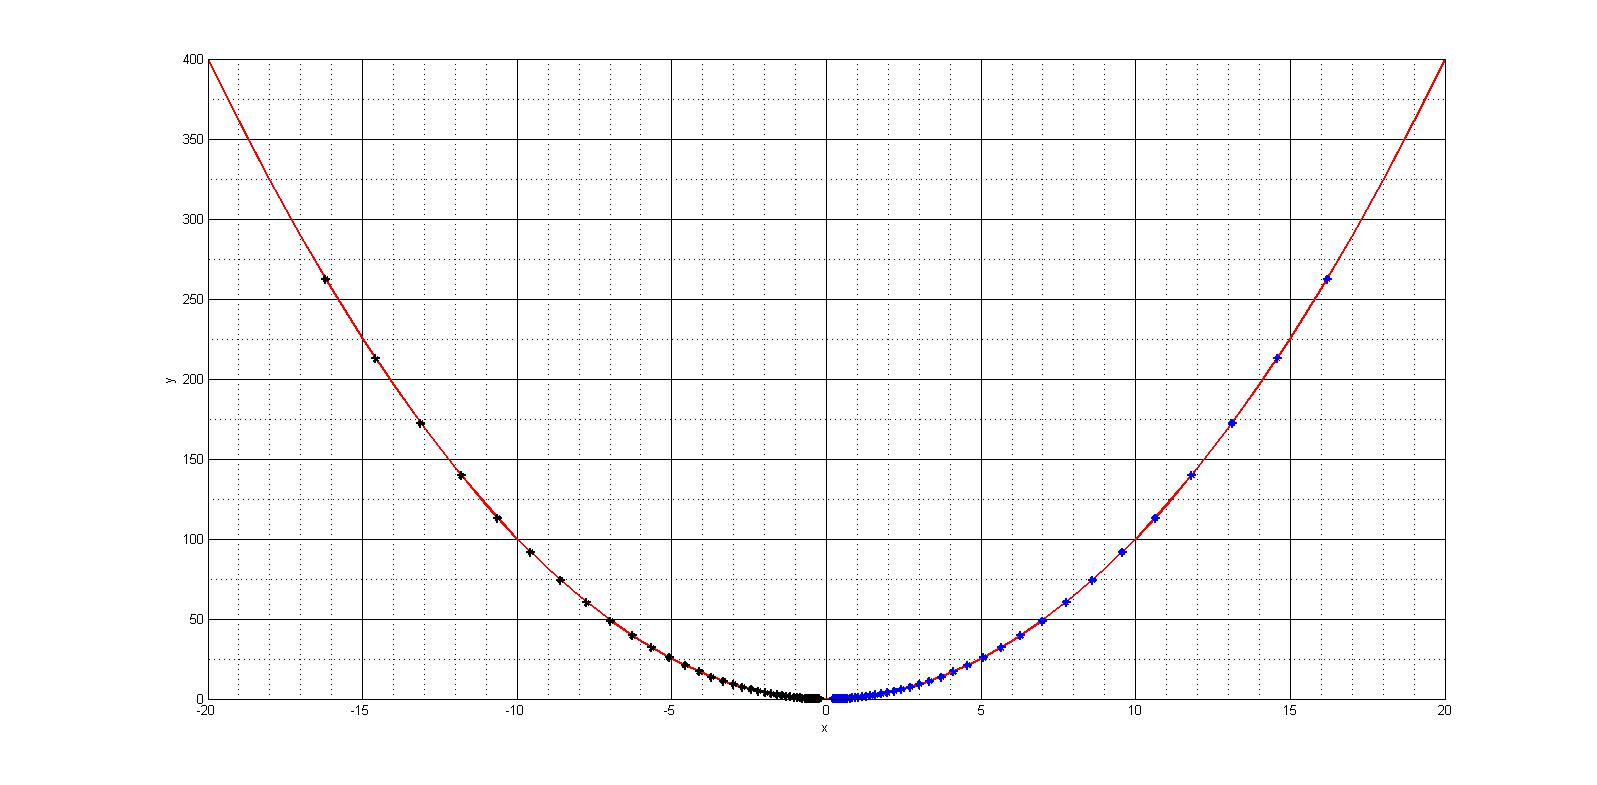
\includegraphics[width=0.8\textwidth]{downhill/Quadrat.jpg}%
  	\caption{Simplex-Downhill auf Quadratfunktion angewendet}%
	\label{fig:SQ1}%
\end{figure}
